% !TeX program = xelatex
\documentclass[a4paper,10pt]{article}

% ============================================================================
% សន្លឹកកិច្ចការសិស្សបំពេញចន្លោះ ស-ខ្មៅ និងប្លង់ក្ដារខៀន/ចម្លើយគ្រូ (គ្មាន LCD / គ្មានកន្ត្រៃ)
% មេរៀនទី១ (៤.១)៖ វិធីបូកនិងវិធីដកនៃចំនួនគត់ — ត្រូវគ្នា ១០០% នឹង LS_Plan_WN12.tex
% ============================================================================
\usepackage[a4paper, left=1.0cm, right=1.0cm, top=0.75cm, bottom=1.00cm, footskip=0.52cm]{geometry}
\usepackage{amsmath}
\usepackage{unicode-math}
\usepackage{fontspec}
\usepackage{array, colortbl}
\usepackage[table]{xcolor}
\usepackage{enumitem}
\usepackage{pifont}
\usepackage{fancyhdr}
\usepackage{lastpage}
\usepackage{tikz}
\usepackage[most]{tcolorbox}
\usetikzlibrary{calc, arrows.meta, decorations.pathreplacing, positioning, babel}

\makeatletter
\let\@expl@@@mark@update@singlecol@structures@@\relax
\makeatother

\providecommand{\NGSFindFonts}{%
  \IfFileExists{C:/Windows/Fonts/cambria.ttc}{%
    \def\NGSSysPath{C:/Windows/Fonts/}%
    \def\NGSUserPath{C:/Users/KIT/AppData/Local/Microsoft/Windows/Fonts/}%
  }{%
    \IfFileExists{./fonts/KhmerOSsiemreap.ttf}{\def\NGSSysPath{./fonts/}\def\NGSUserPath{./fonts/}}{%
    \IfFileExists{../fonts/KhmerOSsiemreap.ttf}{\def\NGSSysPath{../fonts/}\def\NGSUserPath{../fonts/}}{%
    \IfFileExists{../../fonts/KhmerOSsiemreap.ttf}{\def\NGSSysPath{../../fonts/}\def\NGSUserPath{../../fonts/}}{%
    \IfFileExists{../../../fonts/KhmerOSsiemreap.ttf}{\def\NGSSysPath{../../../fonts/}\def\NGSUserPath{../../../fonts/}}{%
    \IfFileExists{../../../../fonts/KhmerOSsiemreap.ttf}{\def\NGSSysPath{../../../../fonts/}\def\NGSUserPath{../../../../fonts/}}{%
    \IfFileExists{../../../../../fonts/KhmerOSsiemreap.ttf}{\def\NGSSysPath{../../../../../fonts/}\def\NGSUserPath{../../../../../fonts/}}{%
    \IfFileExists{../../../../../../fonts/KhmerOSsiemreap.ttf}{\def\NGSSysPath{../../../../../../fonts/}\def\NGSUserPath{../../../../../../fonts/}}{%
      \def\NGSSysPath{../../../../../../../fonts/}\def\NGSUserPath{../../../../../../../fonts/}%
    }}}}}}}%
  }%
}
\NGSFindFonts

\setmathfont[Path={\NGSSysPath}, FontIndex=1, Scale=1.02]{cambria.ttc}
\defaultfontfeatures{Ligatures=TeX}

\setmainfont[
  Path={\NGSUserPath}, Extension=.ttf, Script=Khmer,
  BoldFont={KhmerOSsiemreap}, BoldFeatures={FakeBold=1.8},
  ItalicFont={KhmerOSsiemreap}, ItalicFeatures={FakeSlant=0.25},
  BoldItalicFont={KhmerOSsiemreap}, BoldItalicFeatures={FakeBold=1.8, FakeSlant=0.25}
]{KhmerOSsiemreap}

\newfontfamily\muol[Path={\NGSUserPath}, Extension=.ttf, Script=Khmer]{KhmerOSmuollight}
\newfontfamily\TimesEn[Path={\NGSSysPath}, Extension=.ttf, BoldFont={timesbd}, ItalicFont={timesi}, BoldItalicFont={timesbi}]{times}
\newfontfamily\CalibriFont[Path={\NGSSysPath}, Extension=.ttf]{calibri}

\XeTeXlinebreaklocale "km"
\XeTeXlinebreakskip = 0pt plus 1pt minus 0.1pt

\definecolor{panelgray}{gray}{0.94}
\definecolor{headgray}{gray}{0.85}

\pagestyle{fancy}
\fancyhf{}
\renewcommand{\headrulewidth}{0pt}
\fancyfoot[L]{\fontsize{7.4pt}{9.5pt}\selectfont អនុវិទ្យាល័យព្រះក្រសាំង \en{|} គ្រូ៖ ហុក ប៊ុនថែន \en{|} មេរៀនទី១ (៤.១) វិធីបូកនិងវិធីដកនៃចំនួនគត់ \en{|} ថ្ងៃពុធ ទី៤ ខែវិច្ឆិកា ឆ្នាំ២០២៦}
\fancyfoot[R]{\fontsize{7.8pt}{10pt}\selectfont ទំព័រ \en{\thepage\ / \pageref{LastPage}}}

\setlength{\parindent}{0pt}
\setlength{\parskip}{0pt}
\setlength{\tabcolsep}{4pt}
\newcolumntype{L}[1]{>{\raggedright\arraybackslash}p{#1}}
\newcolumntype{C}[1]{>{\centering\arraybackslash}p{#1}}

\newcommand{\en}[1]{{\TimesEn #1}}
\newcommand{\enbf}[1]{{\TimesEn\bfseries #1}}
\newcommand{\unit}[1]{\,\text{\en{#1}}}
\newcommand{\cnum}[1]{\mbox{\fontsize{10pt}{12pt}\selectfont\ding{\numexpr181+#1\relax}}}
\newcommand{\chkbox}{\tikz[baseline=-0.15ex]\draw[black, line width=0.85pt, fill=white] (0,0) rectangle (0.24cm,0.24cm);}
\newcommand{\ansbox}[1][1.75cm]{\,\tikz[baseline=-0.65ex]\draw[black, line width=0.65pt, fill=white] (0,0) rectangle (#1, 0.42cm);\,}
\newcommand{\dotline}[1][2.2cm]{\makebox[#1]{\dotfill}}

\newcommand{\pagebanner}[2]{%
  \begin{tcolorbox}[
    enhanced, sharp corners, colback=headgray, colframe=black,
    boxrule=1.05pt, boxsep=1pt, top=2.5pt, bottom=2.5pt, left=6pt, right=6pt,
    after skip=3.5pt
  ]
    {\muol\fontsize{9.0pt}{13.2pt}\selectfont #1}\hfill{\fontsize{8.0pt}{11.2pt}\selectfont\textbf{#2}}
  \end{tcolorbox}%
}

\newcommand{\secstrip}[2]{%
  \vspace{3pt}%
  \begin{tcolorbox}[
    enhanced, sharp corners, colback=panelgray, colframe=black,
    boxrule=0.8pt, boxsep=0.8pt, top=2pt, bottom=2pt, left=5pt, right=5pt,
    after skip=3pt
  ]
    {\muol\fontsize{8.5pt}{12.2pt}\selectfont #1}\hfill{\fontsize{7.8pt}{10.8pt}\selectfont\textit{#2}}
  \end{tcolorbox}%
}

\begin{document}
\fontsize{9.5pt}{14.5pt}\selectfont

% ============================================================================
% ទំព័រទី ១៖ សន្លឹកកិច្ចការសិស្ស (ផ្នែកមុខ៖ E1 -> E2 -> E3)
% ============================================================================
\pagebanner{សន្លឹកកិច្ចការសិស្ស \enbf{(}៤\enbf{.}១ វិធីបូកនិងវិធីដកនៃចំនួនគត់\enbf{)} \enbf{--} ផ្នែកមុខ}{ថ្នាក់ទី៧ \en{|} សៀវភៅគោល ទំ.៣--៤}

\begin{tcolorbox}[
  enhanced, sharp corners, colback=white, colframe=black,
  boxrule=0.8pt, boxsep=1.5pt, top=3.5pt, bottom=3.5pt, left=5pt, right=5pt,
  after skip=4pt
]
  \fontsize{9.0pt}{13.0pt}\selectfont
  \textbf{ឈ្មោះសិស្ស៖} \dotline[4.3cm] \quad
  \textbf{សមាជិកក្រុម៖} \dotline[4.3cm] \quad
  \textbf{ថ្នាក់ទី៖} ៧\dotline[0.9cm] \quad
  \textbf{ក្រុមទី៖} \dotline[1.0cm]
\end{tcolorbox}

% --- E1 Engage ---
\secstrip{ផ្នែកទី ១ \enbf{(E1 - Engage)} ៖ បេសកកម្មអន្ទាក់ខ្ចីឆ្លងខ្ទង់សូន្យក្នុង $903 - 347$}{រយៈពេល ៣ នាទី (គូស \ding{51} ក្នុង \chkbox)}

\begin{tcolorbox}[
  enhanced, sharp corners, colback=white, colframe=black,
  boxrule=0.8pt, boxsep=2pt, top=4pt, bottom=4pt, left=6pt, right=6pt
]
  ក្នុងការគណនាផលដក $903 - 347$ (ឧទាហរណ៍ ៣ ក ទំ.៣) សិស្សពីរនាក់ឃើញចម្លើយខុសគ្នា៖\\[3pt]
  $\bullet$ \textbf{តើសិស្សរូបណាគណនាបានត្រឹមត្រូវ?} \quad
  \chkbox\ \textbf{សិស្ស ក៖} $903 - 347 = 566$ \qquad
  \chkbox\ \textbf{សិស្ស ខ៖} $903 - 347 = 556$\\[3pt]
  $\bullet$ \textbf{ផ្ទៀងផ្ទាត់ដោយវិធីបូក៖} $566 + 347 =$ \dotline[1.8cm] \quad រីឯ \quad $556 + 347 =$ \dotline[1.8cm] ។
\end{tcolorbox}

\vfill

% --- E2 Explore ---
\secstrip{ផ្នែកទី ២ \enbf{(E2 - Explore)} ៖ វិធីបូកត្រាទុក វិធីដកខ្ចីឆ្លងសូន្យ និងកសិផលពូសុខ (ទំ.៣--៤)}{រយៈពេល ១១ នាទី}

\textbf{សកម្មភាព ១ (\en{E2-A} — ៥ នាទី)៖ ការតម្រឹមខ្ទង់ក្នុងវិធីបូក និងចំណោទសិស្សសាលា (ឧទាហរណ៍ ១--២ ទំ.៣)}

\begin{tcolorbox}[
  enhanced, sharp corners, colback=white, colframe=black,
  boxrule=0.8pt, boxsep=2.5pt, top=4.5pt, bottom=4.5pt, left=6pt, right=6pt
]
  $\bullet$ \textbf{ឧទាហរណ៍ ១ (ទំ.៣)៖} គណនាផលបូកដោយតម្រឹមខ្ទង់រាយក្រោមរាយ៖\\[3pt]
  \hspace*{0.3cm}ក. $735 + 196 =$ \ansbox[2.0cm] \qquad\qquad
  ខ. $680 + 302 + 96 =$ \ansbox[2.2cm]\\[3.5pt]
  $\bullet$ \textbf{ឧទាហរណ៍ ២ (ទំ.៣)៖} សាលារៀនមួយមានសិស្សថ្នាក់ទី៧ ចំនួន $589$ នាក់ ថ្នាក់ទី៨ ចំនួន $546$ នាក់ និងថ្នាក់ទី៩ ចំនួន $503$ នាក់ ។\\[3pt]
  \hspace*{0.3cm}ចំនួនសិស្សសរុបនៅក្នុងសាលារៀន ៖ $589 + 546 + 503 =$ \dotline[2.4cm] $+ 503 =$ \ansbox[2.2cm] នាក់ ។
\end{tcolorbox}

\vspace{4pt}
\textbf{សកម្មភាព ២ (\en{E2-B} — ៦ នាទី)៖ វិធីដកខ្ចីឆ្លងសូន្យ និងចំណោទកសិផលពូសុខ (ឧទាហរណ៍ ៣--៤ ទំ.៣--៤)}

\begin{tcolorbox}[
  enhanced, sharp corners, colback=white, colframe=black,
  boxrule=0.8pt, boxsep=2.5pt, top=4.5pt, bottom=4.5pt, left=6pt, right=6pt
]
  $\bullet$ \textbf{ឧទាហរណ៍ ៣ (ទំ.៣)៖} បំបែក $903 = 8\text{ រយ} +$ \dotline[0.9cm] $\text{ដប់} + 13\text{ រាយ}$ រួចគណនាផលដក៖\\[3pt]
  \hspace*{0.3cm}ក. $903 - 347 =$ \ansbox[2.0cm] \qquad\qquad
  ខ. $8\,023 - 4\,571 =$ \ansbox[2.2cm]\\[3.5pt]
  $\bullet$ \textbf{ឧទាហរណ៍ ៤ (ទំ.៣--៤)៖} ពូសុខប្រមូលផលសណ្ដែកខៀវនិងសណ្ដែកសៀងសរុប $3\,250\unit{kg}$ ក្នុងនោះសណ្ដែកខៀវមាន $1\,598\unit{kg}$ ៖\\[3pt]
  \hspace*{0.3cm}ម៉ាសសណ្ដែកសៀង ៖ $3\,250 - 1\,598 =$ \ansbox[2.2cm] $\unit{kg}$ \quad (ផ្ទៀងផ្ទាត់៖ $1\,598 +$ \dotline[1.6cm] $= 3\,250\unit{kg}$) ។
\end{tcolorbox}

\vfill

% --- E3 Explain ---
\secstrip{ផ្នែកទី ៣ \enbf{(E3 - Explain)} ៖ ទំនាក់ទំនងច្រាសរវាងវិធីបូក-ដក និងធនាគារហេតុផល \enbf{B\&W}}{រយៈពេល ៦ នាទី}

\begin{tcolorbox}[
  enhanced, sharp corners, colback=white, colframe=black,
  boxrule=0.85pt, boxsep=2.5pt, top=4pt, bottom=4pt, left=6pt, right=6pt
]
  ១) បើ $a + b = c$ នោះ $a = c -$ \dotline[0.9cm] និង $b = c -$ \dotline[0.9cm] \qquad
  ២) បើ $a - b = c$ នោះ $a = c +$ \dotline[0.9cm] និង $b = a -$ \dotline[0.9cm]\\[4pt]
  \tikz\draw[black, dashed, line width=0.5pt] (0,0) -- (18.4cm,0);\\[3.5pt]
  \fontsize{8.8pt}{13.0pt}\selectfont
  \textbf{ធនាគារហេតុផល (\en{Warrant Bank})៖} \quad
  \cnum{1} \textbf{តម្រឹមខ្ទង់៖} រាយក្រោមរាយ ដប់ក្រោមដប់ រយក្រោមរយពីស្ដាំទៅឆ្វេង\\
  \cnum{2} \textbf{ខ្ចីឆ្លងសូន្យ៖} $1\text{ រយ} = 9\text{ ដប់} + 10\text{ រាយ}$ \quad
  \cnum{3} \textbf{ផ្ទៀងផ្ទាត់ច្រាស៖} $a - b = c \iff c + b = a$ \quad
  \cnum{4} \textbf{របារផ្នែក-ទាំងមូល៖} នៅសល់ $=$ សរុប $-$ ស្គាល់
\end{tcolorbox}

% ============================================================================
% ទំព័រទី ២៖ សន្លឹកកិច្ចការសិស្ស (ផ្នែកខាងខ្នង៖ E4 -> E5 -> កិច្ចការផ្ទះ)
% ============================================================================
\clearpage
\pagebanner{សន្លឹកកិច្ចការសិស្ស \enbf{(}៤\enbf{.}១ វិធីបូកនិងវិធីដកនៃចំនួនគត់\enbf{)} \enbf{--} ផ្នែកខាងខ្នង}{ថ្នាក់ទី៧ \en{|} សៀវភៅគោល ទំ.៤ និង ទំ.១៤}

% --- E4 Elaborate ---
\secstrip{ផ្នែកទី ៤ \enbf{(E4 - Elaborate)} ៖ លំហាត់គំរូ — ភ្ញៀវទេសចរទស្សនាប្រាសាទអង្គរវត្តក្នុងរយៈពេល ៣ ខែ (ទំ.៤)}{រយៈពេល ១០ នាទី}

\begin{tcolorbox}[
  enhanced, sharp corners, colback=white, colframe=black,
  boxrule=0.8pt, boxsep=2.5pt, top=4.5pt, bottom=4.5pt, left=6pt, right=6pt
]
  តារាងខាងក្រោមបង្ហាញចំនួនភ្ញៀវទេសចរអន្តរជាតិដែលបានទិញសំបុត្រចូលទស្សនាប្រាសាទអង្គរវត្តក្នុងខែកុម្ភៈ មីនា និងមេសា ។ រកចំនួនភ្ញៀវទេសចរសរុបក្នុងរយៈពេលបីខែ ៖\\[4pt]
  \begin{center}
  {\renewcommand{\arraystretch}{1.25}
  \begin{tabular}{|C{3.8cm}|C{3.8cm}|C{3.8cm}|C{3.8cm}|}
    \hline
    \cellcolor{panelgray}\textbf{ខែ} & \cellcolor{panelgray}\textbf{កុម្ភៈ} & \cellcolor{panelgray}\textbf{មីនា} & \cellcolor{panelgray}\textbf{មេសា} \\ \hline
    \textbf{ចំនួនភ្ញៀវ (នាក់)} & $58\,930$ & $47\,650$ & $73\,280$ \\ \hline
  \end{tabular}}
  \end{center}
  \vspace{3pt}
  $\bullet$ \textbf{ជំហានទី ១ (បូកពីរខែដំបូង \cnum{1})៖} $58\,930 + 47\,650 =$ \dotline[2.4cm] នាក់\\[3.5pt]
  $\bullet$ \textbf{ជំហានទី ២ (បូកសរុបទាំង ៣ ខែ)៖} \dotline[2.2cm] $+ 73\,280 =$ \ansbox[2.5cm] នាក់\\[3pt]
  \fontsize{8.8pt}{12.8pt}\selectfont
  \textbf{ឆ្លុះបញ្ចាំង (\en{EIA Looking-Back})៖} ខែមេសាមានភ្ញៀវច្រើនជាងខែមីនាចំនួន $73\,280 - 47\,650 =$ \dotline[2.0cm] នាក់ ។
\end{tcolorbox}

\vfill

% --- E5 Evaluate ---
\secstrip{ផ្នែកទី ៥ \enbf{(E5 - Evaluate)} ៖ លំហាត់ប្រតិបត្តិ (ទំ.៤) សំណួរវិនិច្ឆ័យ \enbf{A--D} និងសំបុត្រចេញ}{រយៈពេល ១០ នាទី}

\begin{tcolorbox}[
  enhanced, sharp corners, colback=white, colframe=black,
  boxrule=0.8pt, boxsep=2.5pt, top=4.5pt, bottom=4.5pt, left=6pt, right=6pt
]
  \textbf{១) ប្រតិបត្តិជាក្រុមតូច ៣ នាក់ — គណនាផលបូកនិងផលដក (សៀវភៅគោល ទំ.៤)៖}\\[4pt]
  $\bullet$ \textbf{ក.} $46\,382 + 6\,948 + 164\,968 + 1\,896 =$ \dotline[3.0cm] $+$ \dotline[3.0cm] $=$ \ansbox[2.4cm]\\[4.5pt]
  $\bullet$ \textbf{ខ.} $1\,712\,366 - 492\,135 - 54\,201 =$ \dotline[3.2cm] $- 54\,201 =$ \ansbox[2.6cm]\\[4.5pt]
  \textbf{២) បិទបេសកកម្ម \en{E1}៖} សិស្ស \dotline[1.0cm] ត្រឹមត្រូវ ព្រោះ $903 - 347 =$ \dotline[1.5cm] ដោយសារ $556 + 347 =$ \dotline[1.5cm] ។
\end{tcolorbox}

\vspace{4pt}

\begin{tcolorbox}[
  enhanced, sharp corners, colback=white, colframe=black,
  boxrule=0.8pt, boxsep=2.5pt, top=4.5pt, bottom=4.5pt, left=6pt, right=6pt
]
  \textbf{៣) សំណួរវិនិច្ឆ័យ \en{A--D} (តើផលដកឆ្លងសូន្យពីរខ្ទង់ $5\,002 - 1\,645$ ស្មើនឹងប៉ុន្មាន? — គូសរង្វង់ រួចលើកម្រាមដៃ ១--៤)៖}\\[3.5pt]
  \textbf{\en{A.}} $3\,467$ \qquad\qquad\quad
  \textbf{\en{B.}} $3\,357$ \qquad\qquad\quad
  \textbf{\en{C.}} $4\,643$ \qquad\qquad\quad
  \textbf{\en{D.}} $6\,647$\\[4.5pt]
  \tikz\draw[black, dashed, line width=0.5pt] (0,0) -- (18.4cm,0);\\[3.5pt]
  \textbf{៤) សំបុត្រចេញ ៦០ វិនាទី៖} តាមទំនាក់ទំនងច្រាស (\cnum{3}) បើ $x - 1\,408 = 2\,592$ នោះ $x = 2\,592 + 1\,408 =$ \ansbox[2.0cm] ។
\end{tcolorbox}

\vfill

% --- Homework ---
\begin{tcolorbox}[
  enhanced, sharp corners, colback=panelgray, colframe=black,
  boxrule=0.95pt, boxsep=2.5pt, top=4pt, bottom=4pt, left=6pt, right=6pt
]
  {\muol\fontsize{9.0pt}{13.0pt}\selectfont កិច្ចការផ្ទះ \enbf{(}សៀវភៅគោល ទំ.១៤ លេខ ៣\enbf{)}}\\[3pt]
  \fontsize{8.8pt}{13.0pt}\selectfont
  $\bullet$ \textbf{លេខ ៣៖} នៅអនុវិទ្យាល័យមួយមានសិស្សប្រុស $679$ នាក់និងសិស្សស្រី $578$ នាក់ ។ ក្នុងមួយឆ្នាំសិស្សដែលអានសៀវភៅនៅក្នុងបណ្ណាល័យបាន $4$ ក្បាល ឬច្រើនជាង $4$ ក្បាល មានចំនួន $824$ នាក់ ។ តើសិស្សដែលបានអានសៀវភៅនៅក្នុងបណ្ណាល័យតិចជាង $4$ ក្បាលមានចំនួនប៉ុន្មាននាក់?
\end{tcolorbox}

% ============================================================================
% ទំព័រទី ៣៖ ទំព័រគ្រូបង្រៀន (គំរូប្លង់ក្ដារខៀន ៣ ផ្នែក + ចម្លើយផ្ទៀងផ្ទាត់រហ័ស)
% ============================================================================
\clearpage
\pagebanner{ទំព័រគ្រូបង្រៀន ៖ ប្លង់ក្ដារខៀន \enbf{(}គ្មាន \enbf{LCD)} និងចម្លើយផ្ទៀងផ្ទាត់រហ័ស}{៤.១ វិធីបូកនិងវិធីដកនៃចំនួនគត់ (\en{WN12})}

\secstrip{១. គំរូប្លង់បែងចែកក្ដារខៀន ៣ ផ្នែក សម្រាប់ថ្នាក់រៀនគ្មាន \enbf{LCD}}{សម្រាប់គ្រូប្រើដីស/ហ្វឺត}

\begin{center}
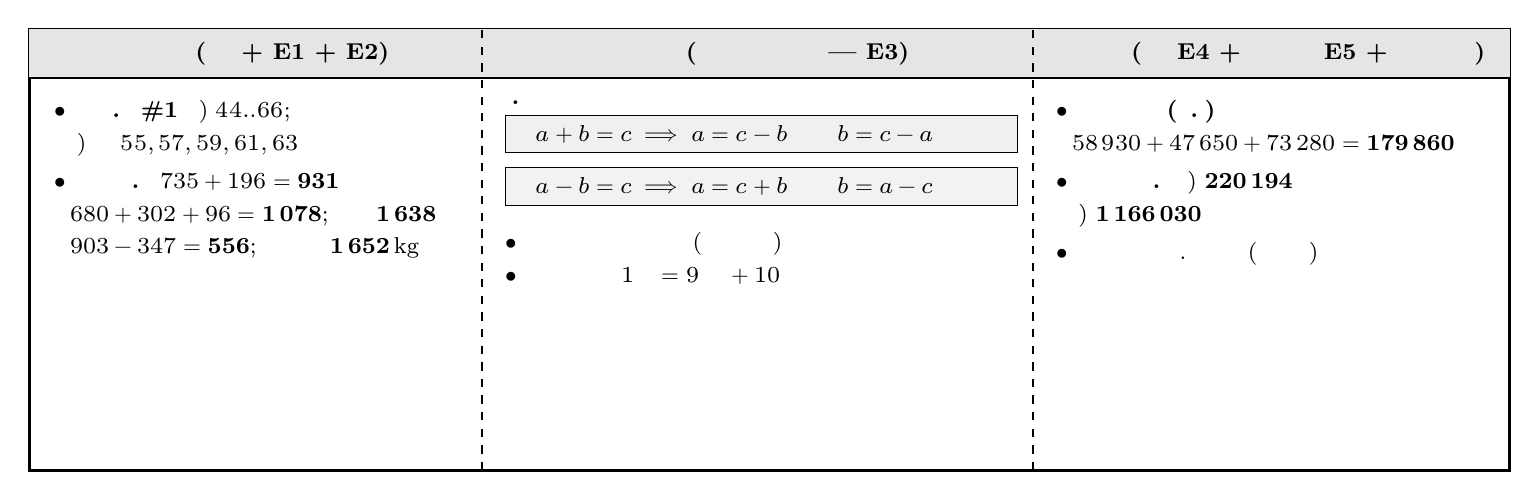
\begin{tikzpicture}[x=1cm, y=1cm, every node/.style={font=\fontsize{8.3pt}{11.8pt}\selectfont, text=black}]
  \draw[black, line width=1.1pt] (0,0) rectangle (18.8,5.60);
  \fill[gray!20] (0,4.98) rectangle (18.8,5.60);
  \draw[black, line width=0.7pt] (0,4.98) -- (18.8,4.98);
  \draw[black, dashed, line width=0.7pt] (5.75,0) -- (5.75,5.60);
  \draw[black, dashed, line width=0.7pt] (12.75,0) -- (12.75,5.60);

  \node at (2.875,5.29) {\textbf{ផ្នែកឆ្វេង (កំណែ + \en{E1} + \en{E2})}};
  \node at (9.25,5.29) {\textbf{ផ្នែកកណ្ដាល (ខ្លឹមសារគោលរក្សាទុក — \en{E3})}};
  \node at (15.775,5.29) {\textbf{ផ្នែកស្ដាំ (គំរូ \en{E4} + ប្រតិបត្តិ \en{E5} + កិច្ចការផ្ទះ)}};

  % Left
  \node[anchor=north west, text width=5.35cm] at (0.20,4.82) {%
    $\bullet$ \textbf{កំណែទំ.១៤ \#1៖} ក) $44..66$;\\
    \hspace*{0.2cm}ខ) សេស $55, 57, 59, 61, 63$\\[2pt]
    $\bullet$ \textbf{ឧទាហរណ៍ទំ.៣៖} $735+196=\mathbf{931}$\\
    \hspace*{0.2cm}$680+302+96=\mathbf{1\,078}$; សិស្ស $\mathbf{1\,638}$\\
    \hspace*{0.2cm}$903-347=\mathbf{556}$; សណ្ដែកសៀង $\mathbf{1\,652\unit{kg}}$
  };

  % Center
  \node[anchor=north west, text width=6.65cm] at (5.92,4.82) {%
    {\muol\fontsize{8.5pt}{12pt}\selectfont ៤\enbf{.}១ វិធីបូកនិងវិធីដកនៃចំនួនគត់}\\[3pt]
    \tikz\node[draw=black, fill=gray!12, inner sep=3.5pt, text width=6.25cm]{%
      បើ $a + b = c \implies a = c - b$ \ និង \ $b = c - a$
    };\\[4pt]
    \tikz\node[draw=black, fill=gray!10, inner sep=3.5pt, text width=6.25cm]{%
      បើ $a - b = c \implies a = c + b$ \ និង \ $b = a - c$
    };\\[4pt]
    $\bullet$ តម្រឹមខ្ទង់ពីស្ដាំទៅឆ្វេង (រាយក្រោមរាយ)\\
    $\bullet$ ខ្ចីឆ្លងសូន្យ៖ $1\text{ រយ} = 9\text{ ដប់} + 10\text{ រាយ}$
  };

  % Right
  \node[anchor=north west, text width=5.65cm] at (12.92,4.82) {%
    $\bullet$ \textbf{គំរូអង្គរវត្ត (ទំ.៤)៖}\\
    \hspace*{0.2cm}$58\,930 + 47\,650 + 73\,280 = \mathbf{179\,860}$ នាក់\\[2pt]
    $\bullet$ \textbf{ប្រតិបត្តិទំ.៤៖} ក) $\mathbf{220\,194}$\\
    \hspace*{0.2cm}ខ) $\mathbf{1\,166\,030}$\\[2pt]
    $\bullet$ \textbf{កិច្ចការផ្ទះ៖} ទំ.១៤ លេខ ៣ (បណ្ណាល័យ)
  };
\end{tikzpicture}
\end{center}

\vfill
\secstrip{២. ចម្លើយផ្ទៀងផ្ទាត់រហ័សសម្រាប់សន្លឹកកិច្ចការសិស្ស \enbf{(}ទំព័រ ១ និង ទំព័រ ២\enbf{)}}{\en{Answer Key}}

\begin{tcolorbox}[
  enhanced, sharp corners, colback=white, colframe=black,
  boxrule=0.8pt, boxsep=2.5pt, top=4.5pt, bottom=4.5pt, left=6pt, right=6pt
]
  \fontsize{9.0pt}{13.6pt}\selectfont
  $\bullet$ \textbf{ផ្នែក \en{E1}៖} \textbf{សិស្ស ខ} ត្រឹមត្រូវ ($556$) ព្រោះ $566 + 347 = 913 \ne 903$ រីឯ $556 + 347 = 903$ ។\\[2.5pt]
  $\bullet$ \textbf{ផ្នែក \en{E2}៖} \textbf{សកម្មភាព ១៖} ក) $931$, ខ) $1\,078$; ឧទាហរណ៍ ២៖ $1\,135 + 503 = 1\,638$ នាក់ ។ \textbf{សកម្មភាព ២៖} $8\text{ រយ} + 9\text{ ដប់} + 13\text{ រាយ} \implies$ ក) $556$, ខ) $3\,452$; ពូសុខ៖ $1\,652\unit{kg}$ ។\\[2.5pt]
  $\bullet$ \textbf{ផ្នែក \en{E4}៖} ជំហាន ១៖ $106\,580$ នាក់; ជំហាន ២៖ $106\,580 + 73\,280 = 179\,860$ នាក់; \en{EIA}៖ $25\,630$ នាក់ ។\\[2.5pt]
  $\bullet$ \textbf{ផ្នែក \en{E5}៖} \textbf{១) ប្រតិបត្តិ៖} ក) $53\,330 + 166\,864 = 220\,194$; ខ) $1\,220\,231 - 54\,201 = 1\,166\,030$ ។ \textbf{២) បិទ \en{E1}៖} សិស្ស ខ ($556$, $903$) ។ \textbf{៣) វិនិច្ឆ័យ \en{A--D}៖} \textbf{ជម្រើស \en{B}} ($3\,357$) ។ \textbf{៤) សំបុត្រចេញ៖} $x = 4\,000$ ។
\end{tcolorbox}

\vfill
\secstrip{៣. ចម្លើយលម្អិតនៃកិច្ចការផ្ទះ \enbf{(}សៀវភៅគោល ទំ.១៤ លេខ ៣\enbf{)}}{សៀវភៅគោល ទំ.១៤}

\begin{tcolorbox}[
  enhanced, sharp corners, colback=white, colframe=black,
  boxrule=0.8pt, boxsep=2.5pt, top=4.5pt, bottom=4.5pt, left=6pt, right=6pt
]
  \fontsize{8.9pt}{13.4pt}\selectfont
  $\bullet$ \textbf{លេខ ៣ (ទំ.១៤ — សិស្សប្រុស $679$ នាក់ សិស្សស្រី $578$ នាក់; អានសៀវភៅ $\ge 4$ ក្បាលមាន $824$ នាក់)៖}\\[2.5pt]
  \hspace*{0.3cm}១) ចំនួនសិស្សសរុបនៅក្នុងអនុវិទ្យាល័យ៖ $679 + 578 = \mathbf{1\,257\text{ នាក់}}$ ។\\[2pt]
  \hspace*{0.3cm}២) ចំនួនសិស្សដែលអានសៀវភៅតិចជាង $4$ ក្បាល៖ $1\,257 - 824 = \mathbf{433\text{ នាក់}}$ (ផ្ទៀងផ្ទាត់៖ $824 + 433 = 1\,257$ នាក់) ។
\end{tcolorbox}

\vfill
\secstrip{៤. ចំណុចប្រុងប្រយ័ត្នគរុកោសល្យសម្រាប់គ្រូ \enbf{(}ការយល់ច្រឡំសំខាន់ៗ និងវិធីកែតម្រូវភ្លាមៗ\enbf{)}}{\en{Pedagogical Watchlist}}

\begin{tcolorbox}[
  enhanced, sharp corners, colback=panelgray, colframe=black,
  boxrule=0.85pt, boxsep=2.5pt, top=4.5pt, bottom=4.5pt, left=6pt, right=6pt
]
  \fontsize{8.8pt}{13.2pt}\selectfont
  $\bullet$ \textbf{អន្ទាក់ទី ១ (ការខ្ចីរំលងខ្ទង់សូន្យ — \en{Brown \& VanLehn, 1982})៖} ក្នុង $903 - 347$ ឬ $5\,002 - 1\,645$ ចូរឱ្យសិស្សសរសេរលេខខ្ចីពីលើខ្ទង់ ($4\ \,9\ \,9\ \,12$ លើ $5\,002$) និងប្រើវិធីបូកច្រាសត្រួតពិនិត្យភ្លាមៗ ។\\[2.5pt]
  $\bullet$ \textbf{អន្ទាក់ទី ២ (ការដកបន្តពីរតួក្នុងប្រតិបត្តិ ខ)៖} ក្នុង $1\,712\,366 - 492\,135 - 54\,201$ ត្រូវដកតាមលំដាប់ពីឆ្វេងទៅស្ដាំ (យកលទ្ធផលដកទី១ ទៅដកនឹង $54\,201$) កុំយក $492\,135 - 54\,201$ មុនឱ្យសោះ!
\end{tcolorbox}

\end{document}
